\documentclass[12pt]{article}
\usepackage{graphicx}
\usepackage{subcaption}
\usepackage{amsfonts}
\usepackage{amsmath}
\usepackage{fullpage}
\usepackage[utf8x]{inputenc}
\makeatletter
\usepackage{cite}
\usepackage{hyperref}
\@namedef{opt@inputenc.sty}{utf8}
\makeatother
\usepackage{url}    
\usepackage{CJKutf8}
\usepackage{multirow}
\usepackage{array}
\newenvironment{conditions}
  {\par\vspace{\abovedisplayskip}\noindent\begin{tabular}{>{$}l<{$} @{${}={}$} l}}
  {\end{tabular}\par\vspace{\belowdisplayskip}}
\begin{document}
\title{
\begin{flushright}
\includegraphics[width=2.5cm]{logoUHi.jpg}\\
{\small
Data Analytics\\
Stiftung Universit{\"a}t Hildesheim\\
Marienburger Platz 22\\
31141 Hildesheim\\
Prof. Dr. Dr. Lars Schmidt-Thieme\\
}
\end{flushright}
\bigskip
\begin{center}
Thesis\\
Unsupervised Real-Time Time-Series Anomaly Detection\\
\end{center}
}
\author{Abdul Rehman Liaqat}
\date{271336, Liaqat@uni-hidesheim.de}
\maketitle

\newpage

\begin{abstract}
Anomaly detection is a crucial task for machine learning due to wide-spread usage and type. In particular, it is worth noting that most data arising in industrial setups are of a streaming nature, thus restricting the range of standard anomaly detection tools. This thesis will identify the potential approaches to learn the identification of abnormal behavior from large-scale streaming data. An empirical comparison of state-of-the-art methods will to be extended by a novel technical contribution. In this thesis, the focus is particularly on streaming time-series Anomaly Detection which changes in nature with time and novel contribution will especially try to target this dynamic nature of time-series.
\end{abstract}
\newpage
\tableofcontents
\newpage
\section{Introduction 10 pages}
\begin{enumerate}
	\item Usage of streaming data		
	\item Usage of anomaly detection in general
	\item Software2.0 development and anomaly detection role
	\item Usage of anomaly detection in streaming data
	\item problems in the concept and brief intro to our innovation
\end{enumerate}
\subsection{Usage of streaming data}
With the increase in networking of objects, amount of data being generated is increasing. A big chunk of this data involves streaming data. Streaming data can be defined as data being generated continuously or with a continuous time interval. Statistically, IoT data has grow from 4.4ZB (Zeta Bytes) to 44.4ZB with 50 billions devices. These devices include a small temperature sensor installed in a room to ECG data to satellite communication data. Even videos are kind of streaming data since they include data points (frames) separated by a constant interval. 
\subsection{Usage of anomaly detection in general}
An anomaly is defined as significantly different data point from other data points. The difference is dependent upon the at least two things. One is the data point being an outlier in general among all data points available. Second is that the data point value doens't make sense in the sequence data is being generated hence it is possible for new data point to be extremely different from all previous ones but still make sense to have in the sequence and vice versa. Detecting an anomaly helps in identifying abnormal behavior of a process with potentially useful information. 
\subsection{Software2.0 development and anomaly detection role}
As described in (reference name Software2), going forward software development especially machine learning based software development will be divided into two parts. One part is the preparation of the data and the second part is the design and optimization of algorithms. Both of these steps are used iteratively. Interestingly, as described in the (reference name Software2), more and more time is spent on accumulating, massaging and cleaning datasets. One major part of this process is outlier detection, anomaly detection and novelty detection. By detection of anomalies, it will become sufficiently easy for human expert to find the one data point in a heap of millions data points and then decide whether to remove that data or get more of the same data points.
Need of an anomaly detection algorithm to identify faulty devices or prevent potential system failure before it happens. Thus the anomaly detection algorithm should be generic (unsupervised), be ready to predict on live data and be able to consider the important past data points (temporal and spatial pattern detection).
\subsection{Usage of anomaly detection in streaming data}
\subsection{problems in the concept and brief intro to our innovation}
Now to define the problem officialy, time series can be defined as an ordered sequence of values of a variable at equally spaced time intervals. It can be a variable or group of variables. For example a heat sensor will be producing one time series which is why it is called univariate time series. If we also consider the output of humidity sensor and noise sensor then the group of these univariate time series will be called multivariate time series. Usually techniques applied on univariate time series can also be used on multivariate after some modification. That's why we will be focusing on univariate time series only in this research thesis. \\
\break
A streaming data or streaming time series has some properties specialized to it. A univariate streaming time series will have following properties:
\begin{enumerate}
	\item Every new data point $x_t$ will be following by a new data point $x_{t+1}$
	\item The time difference between $t - (t-1)*$ and $(t+1) - t$ is approximately the same
	\item There is no known ending time of the stream hence making the streaming data a major source of big data. With this requirement it becomes important to identify important part or time range of the series to be used for the processing.  
\end{enumerate}
Moving on there are some unique concepts related to uni-variate time series which will be helpful in the understanding of the research problem. Starting with stationary and non-stationary time series. A stationary time series is the one whose statistical properties are constant over time. These statistical properties include mean, variance and auto-correlation of the time series. Similarly with the change in one or more of these statistical properties, non-stationary time series comes into being. These non-stationary time series are also named as Concept drift. Concept drift is a terminology related to time series data specifically which is why we will be using the term Concept drift instead of non-stationary time series in future. There is also an intuitive meaning behind the name of Concept drift.\\
\break
Considering that there is an underlying probability distribution in every time series and this underlying distribution is named Concept of time series such as
\begin{equation}
Concept =  P_t(X)
\end{equation} 
The the concept drift occurs between two times t and u when the distribution or concept changes as
\begin{equation}
    P_t(X) \neq P_u(X)
\end{equation}
And the new data points are generated from the second distribution $p_u(X)$ onward rather then the original $P_t(X)$ for a length of time $T$. This time $T$ is decided by the domain knowledge and frequency of data points.
As in real life systems it is highly likely that there will be a change in the concept of the time-series hence happening of concept drift is very likely and possible. For example, there will be a concept drift in the time-series output of a heat sensor measuring the temperature of a motor of exhaust fan and the motor of the fan is changed. Thus it is necessary for our system to first recognize the concept drift. If there exists a concept drift then the model should adapt itself swiftly to avoid false positives. Similarly if there is not a concept drift then the model should not give much learning weight to these readings. Thus the model adaption according to presence of concept drift is necessary.\\
\break
Time series data is the output of a streaming data from multiple devices which makes it close to impossible to label it specially for anomalies. Also due to concept drift a regular labeling needed. Since it is very difficult to label streaming time series data to detect anomalies it makes sense to do it in an unsupervised fashion. With unsupervised anomaly detection we don't need any previous labeled data and the system developed will be very generic.
An anomaly is defined as a data point $X_t$ or set of data points $X_{t-l:t}$ for which either of following is true
$\gg \ll$ Example of each anomaly
\begin{enumerate}
    \item Probability of point $X_t$ belonging to a probability distribution $\phi$ is very less then the probability of previous data points $X_n$ where $n \leq t-1$. In other words:\\
    \begin{equation}
        P(X_t) \in \phi  \ll P(X_n) \in \phi 
    \end{equation}
    This type of anomaly is called point anomaly. Here $\phi$ is the probability distribution generating all the data points.
    \item Probability of points $X_{t-l:t}$ belonging to a probability distribution $\phi$ is very less then the probability of $X_{n-l:n}$ where $n \leq t-1$. In other words: \\
    \begin{equation}
        P(X_{t-l:t}) \in \phi  \ll P(X_{n-l:n}) \in \phi         
    \end{equation}
        This type of anomaly is called collective anomaly.
    \item Probability of point $X_t$ belonging to a probability distribution $\phi$ is almost same as the probability of previous data points $X_n$ where $n \leq t-1$ but the probability of point $X_t$ belonging to a probability distribution $\theta$ is very less than the probability of point $X_p$ belonging to $\theta$. Here In other words:\\
    \begin{equation}
        P(X_t) \in \phi  \approx P(X_n) \in \phi 
    \end{equation}
    \begin{equation}
        P(X_t) \in \theta  \ll P(X_n) \in \theta 
    \end{equation}
    Here $\theta$ and  $X_p$ are probability distribution and data points. $theta$ is a distribution defined to a set of local points $X_p$ where $p \leq t$ and $p$ is a set of indices. 
    This type of anomaly is called Contextual anomaly. 
\end{enumerate}
Now to detect all the type of anomalies described above it is necessary to estimate the underlying probability distributions responsible for generating the stream. In general there are following few steps in an Anomaly detection framework as described in figure \ref{generalAnomalyDetectionFrameWork}.\\
\break
First step is to pre-process the input data. We use min-max normalization to make sure that all input values are limited between $0$ and $1$. Min-max normalization can be defined as
\begin{equation}
    z = \frac{x - min(x)}{max(x) - min(x)}
\end{equation}
Second step is to estimate the underlying probability distribution by building a model. This model can be used to model the streaming time series. \\
\break
Next step would be to score the incoming data point. At this moment we will use the previously estimated probability distribution and types of anomalies defined above to score the incoming data point. \\
\break
Afterwards the score is passed through a post-processing step. In this step possibly normalization and probabilistic likelihood estimation is applied on top of the previously calculated anomaly score. In other words previously calculated anomaly score is transformed between the range of $0$ and $1$. \\
\break
After post-processing, we can use this score to actually rank each incoming data point among previously existing data points. To label each data point as anomaly or not anomaly a thresholding procedure is necessary. Depending upon the type of post-processing extreme cases are considered as anomalies.
\begin{figure}
\centering
        \includegraphics[width=\textwidth]{images/generalAnomalyDetectionFrameWork.png}
    \caption{General Anomaly Detection Framework}
    \label{generalAnomalyDetectionFrameWork}
\end{figure}
Thus there are many possible points of innovation in the anomaly detection framework based upon the type of problem we are facing. A quick brief of these likely innovations are following:
\begin{enumerate}
    \item First possible innovation is done at the pre-processing step. Here it is very helpful to normalize the input data and constrain it between $0$ and $1$. The benefits of normalization show up while calculating anomaly score as anomaly score will be then close to the range of $0$ and $1$. Another very important point is  
    \item Second and a major problem to solve is the algorithm that will estimate the probability distribution of streaming data. This algorithm should have at least following properties:
    \begin{itemize}
    	\item The algorithm should have the capability to differentiate the concept drift with actual anomalies and adapt itself accordingly.
    	\item The algorithm cannot look ahead in the future values. In other words the algorithm will work on real-time streaming data and will only be dependent upon current and past values.
    	\item It should be able to train itself ideally, before the arrival of next data point. This condition will make the algorithm fast and online.
    \end{itemize}
	\item Another possible innovation area is the values the algorithm is trained for. The algorithm can be an autoencoder based and be used to reconstruct a window of current and past values hence predicting a sequence which will then be compared with original values. The distance between the predicted sequence of reconstruction and actual values will be used as anomaly score then. Otherwise using a sub-sequence, one can predict another sub-sequence which is few time step ahead of the input sequence. The autoencoder learns how to reconstruct the current sequence and predictive learns how to predict the future values. 
	\item Now that we have an anomaly score, next step is to apply some post-processing on top of this score. There are two possible variations used. First variation is moving min-max normalization. With this kind of normalization current point is normalized by using the minimum and maximum values of the data obtained so far. Seoncd type of post-processing is probability of values of a current small window from the previous values.
\end{enumerate}
\newpage
\section{Related Work and State of the art 10 pages}
\begin{enumerate}
	\item Time series intro. Prediction and classification.
	\item Unsupervised methods on time series 
	\item Anomaly detection
	\item Time series Anomaly detection
	\item Unsupervised Time series Anomaly detection
	\item General components latest anomaly detection methods and explanation of each
	\item HTM based anomaly detection paper review. Problems or way it does it
	\item paper 2
	\item paper 3
	\item general review, problems, bottlenecks and trend
\end{enumerate}
\newpage
\section{Proposed method 10 pages}
\subsection{General anomaly score based architecture and detailed explanation}
\begin{figure}
\centering
        \includegraphics[width=\textwidth]{images/generalAnomalyDetectionFrameWork.png}
    \caption{General Anomaly Detection Framework}
    \label{generalAnomalyDetectionFrameWork}
\end{figure}
Considering figure ~\ref{generalAnomalyDetectionFrameWork}, each algorithm will be using  
all parts with few variations and a cusotmized algorithm part.\\
\break
Pre-processing is playing crucial role in the generalization of the algorithms. There are two different kind of normalization techniques tested. First kind is global normalization
Proposed method can be divided in multiple parts. First part would be the implementation of baselines using latest deep learning architectural components. We use these components to develop two different kind of detectors.\\
\break
One detector is based upon prediction of a next data point. Let $T_{(t-L-1):(t-1)}$ is the small window taken from time series. The starting point is $t-L-1$ where $L$ is the window size and last data point is taken from $t-1$ which is the data point at previous time step. This data window is used to predict the time series value at time $t$. To predict at time $t$ various different kind of functions as baselines using latest architectural components are designed. Generally the output of such a function would be
\begin{equation}
f(T_{(t-L-1):(t-1)}) = \hat{f}(t)
\end{equation} 
Thus the function $f$ in prediction based models map data points as: $f: L \mapsto 1$ where $L$ is the window size and output is the prediction of value at current time. For optimization of function $f$, the difference between time series value at current time step and predicted value at current time is taken. More specifically the objective function will be
\begin{equation}
min |\hat{f}(t) - f(t)|
\end{equation}
That is to minimize the difference between time series value at time $t$ and predicted time series value at time $t$ using time series value from $T_{(t-L-1):(t-1)}$.
\subsection{Describe autoencoder based architecture}
An autoencoder is a network which is trained to copy its input to its output, with the typical purpose of dimension reduction - the process of reducing the number of random variables under consideration. It features an encoder function to create a hidden layer (or multiple layers) which contains a code to describe the input. There is then a decoder which creates a reconstruction of the input from the hidden layer. An autoencoder can then become useful by having a hidden layer smaller than the input layer, forcing it to create a compressed representation of the data in the hidden layer by learning correlations in the data. This compressed representation is actually summarized version of input. This way for the anomaly input values, summarized version will not output very similar output and hence ending up creating big reconstruction loss.
The backpropagation will try to  $h_{W,b}(x) \approx x$ , so as to minimise the mean square difference:
\begin{equation}
L(x,y) = \sum(x-h_{W,b}(x))^2
\end{equation}
Similarly for time series let $X_t$ be the input value of the streaming data at time $t$ then the input of autoencoder based architecture will be $X_{t-w:t}$ and output will be $Y_{t-w:t}$ as $Y$ is the predicted reconstruction of the input. 
\begin{equation}
Y_{t-w:t} = h(X_{t-w:t})
\end{equation}
The reconstruction loss is defined as:
\begin{equation}
L(x,y) = \frac{1}{w}\sum(Y_{t-w:t}-X_{t-w:t})^2
\end{equation}
$\gg \ll$ picture of an autoencoder
\subsection{Describe Multistep-Ahead based architecture}
$\gg \ll$ picture of an multi-step based architecture
Second type of architecture used is multi-step prediction architecture. In this type of architecutre 
For time series let $X_t$ be the input value of the streaming data at time $t$ then the input of multistep prediction based architecture will be $X_{t-w-l:t-l}$ and output will be $Y_{t-l:t}$ as $Y$ is the prediction of the input. 
More specifically
\begin{equation}
Y_{t-l:t} = h(X_{t-w-l:t-l})
\end{equation}
and the prediction loss will be defined as:
\begin{equation}
L(x,y) = \frac{1}{l}\sum(Y_{t-l:t}-h(X_{t-w-l:t-l}))^2
\end{equation}

Above two are the basic outputs which are repeated with following different architectures.
\subsection{Describe fully connected architecture}
\begin{figure}
\centering
        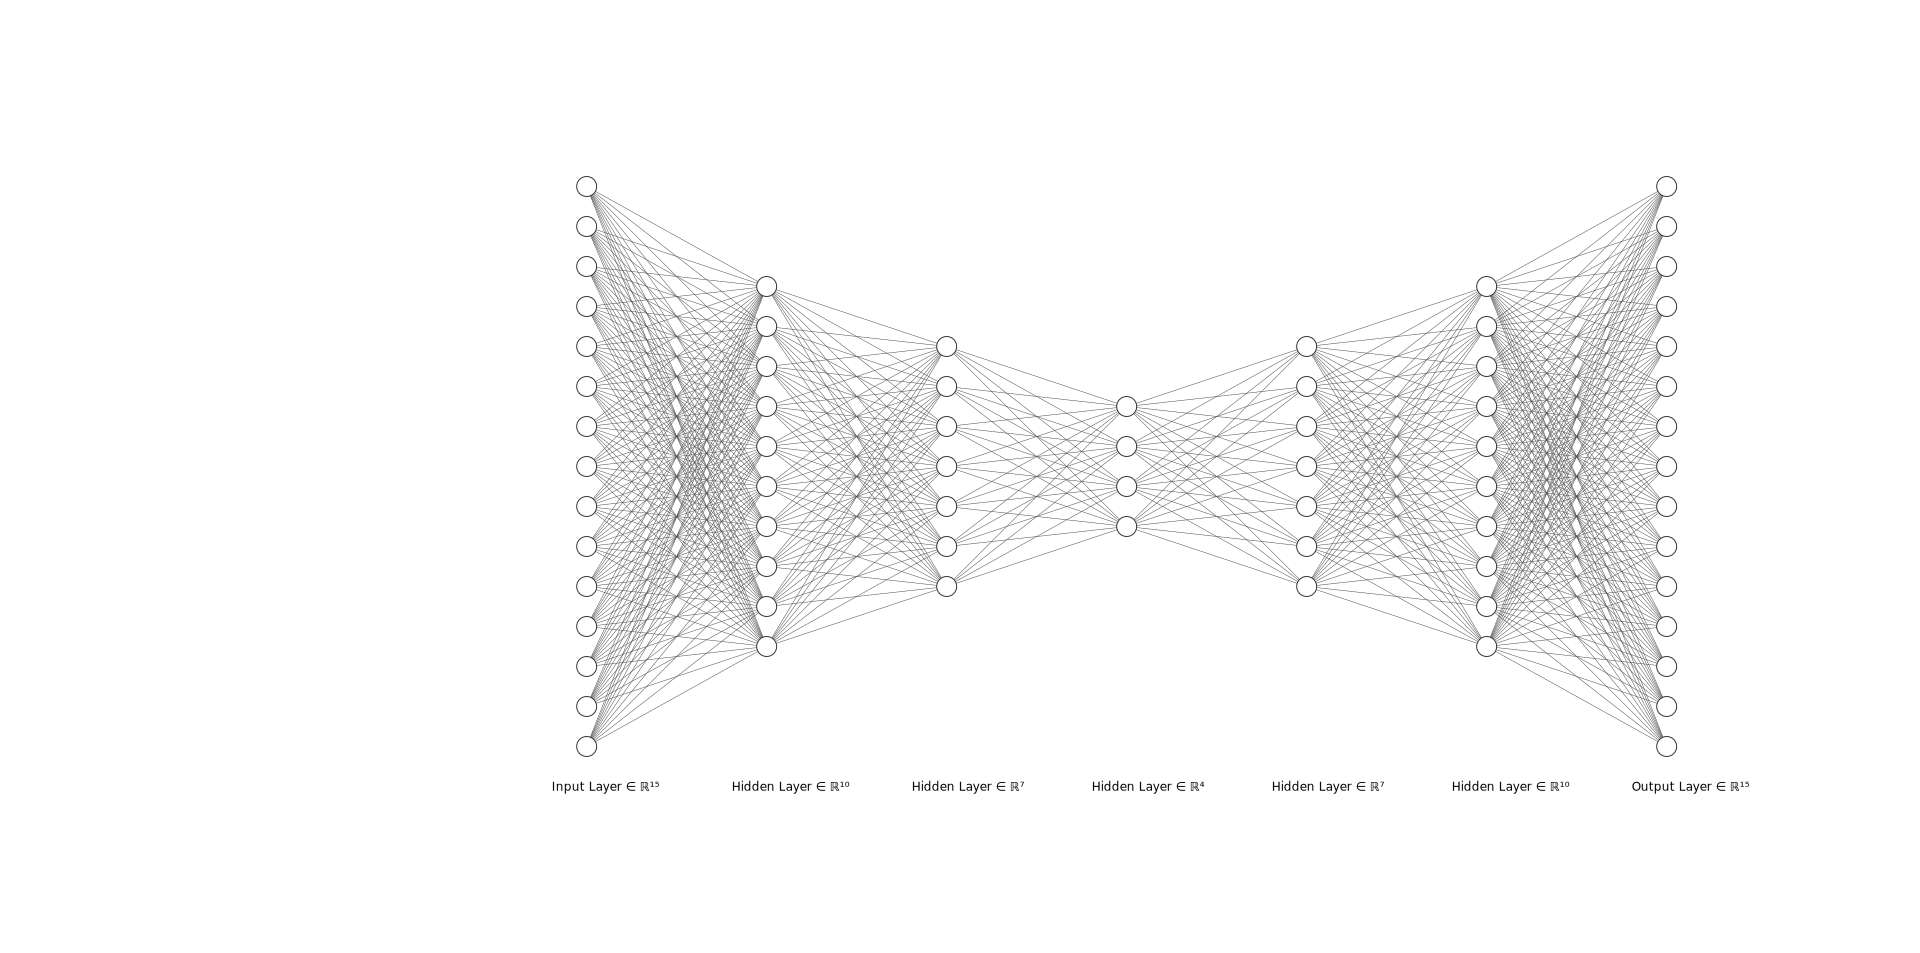
\includegraphics[width=\textwidth]{images/nn.png}
    \caption{Fully connected autoencoder}
    \label{generalAnomalyDetectionFrameWork}
\end{figure}
\subsection{Describe fully connected prediction architecture}
\subsection{Describe fully connected autoencoder architecture}
\subsection{Describe Convolution based prediction architecture}
\subsection{Describe LSTM based prediction architecture}
\subsection{Describe LSTM based autoencoder based architecture}
\subsection{Recency concept}
\subsection{Post-processing}
\subsection{Thresholding}
\subsection{Parameterinzing the anomaly score}
\newpage 
\section{Empirical Formulation and Experiments 5 pages}
To experiment with proposed method and campare them with state-of-the-art results Numenta Anomaly Benchmark (NAB) was used. Numenta is a benchmark specifically designed for online time series anomaly detection.\\
\break
Using NAB provides with many benefits. First is a benchmark dataset which $58$ various univariate time series, each with timestamp as index and value. Length of each time series ranges from $1000$ to $22000$ data points. These $58$ time series are from six different categories. These categories include artificially generated time series, times series gathered from advertisement industry related data such as click through rate (CTR), AWS usage metrics, server traffic data, tweets volume time series and known cause anomaly which has the a solid reason for the labeled anomaly.\\
\break
The diversity of these categories provide the second benefit. With the diversity almost all type of anomalies are covered hence each algorithm can be tested against each type. Artificial datasets further contains time series with anomalies and without anomalies. Datasets without anomalies contain only normal patterns and no anomaly thus any predicted anomaly will be a false positive here. 

\begin{figure}
  \begin{subfigure}[t]{.5\textwidth}
    \centering
    \includegraphics[width=\linewidth]{images/dataAnomalies/artificial/art_daily_flatmiddle.png}
    \caption{Artificial with sudden flat-middle}
  \end{subfigure}
  \hfill
  \begin{subfigure}[t]{.5\textwidth}
    \centering
    \includegraphics[width=\linewidth]{images/dataAnomalies/artificial/art_daily_jumpsdown.png}
    \caption{Artificial with sudden jumps-down}
  \end{subfigure}

  \medskip

  \begin{subfigure}[t]{.5\textwidth}
    \centering
    \includegraphics[width=\linewidth]{images/dataAnomalies/artificial/art_daily_jumpsup.png}
    \caption{Artificial with sudden jumps-up}
  \end{subfigure}
  \hfill
  \begin{subfigure}[t]{.5	\textwidth}
    \centering
    \includegraphics[width=\linewidth]{images/dataAnomalies/artificial/art_daily_nojump.png}
    \caption{Artificial with sudden flat}
  \end{subfigure}
  \caption{Examples of artifical anomaly data set}
  \label{lane_detection}
\end{figure}



\subsection{Dataset}
\newpage
\section{Results 10 pages}
\subsection{Scoring}
\subsection{Comparing with others}
\newpage
\section{Conclusion and Discussion 5 pages}
\newpage
\section{Experiment Infrastructure}
\newpage
\subsection{Experiment Management using MLflow}
\newpage
\subsection{Parallel execution using Docker}
\newpage
\section{Best practices}
Following steps were taken to maximize the efficiency and speed of research:
\begin{enumerate}
	\item Use version control to track the code and share between different devices.
	\item Separate code from data. This will keep the code base small and easy to debug.
	\item Separate input data,working data and output data.
	\begin{itemize}
		\item \textbf{Input Data:} Input data-set that never change. For my case it is NAB and other external datasets.
		\item \textbf{Working Data:} nothing for now.
		\item \textbf{Output Data:} Results and threshold profiles in my case. 
	\end{itemize}
	\item Separate options from parameter. This is important:
 	\begin{itemize}
 		\item Options specify how your algorithm should run. For example data path, working directory and result directory path, epochs, learning rate and so on.
 		\item parameters are the result of training data. it includes the score and hyper-parameters. 
 	\end{itemize}
	
\end{enumerate}
\newpage
\subsection{Moving from jupyterlab to pycharm}
While working with jupyterlab notebook following routine was followed:
1- Load data with sample function
2- Write an algorithm
3- Test the results
4- Write general executeable .py file.
5- Get results on server

Since we needed to track change on two different places,
it was becoming harder to track the bugs and improve on efficiency.
That's why pycharm was selected to create executeable files and test
algorithms at the same time.
\section{Reference Usage}
\newpage
\section{References}
\begingroup
\nocite{*}
\renewcommand{\section}[2]{}
\bibliographystyle{IEEEtrans}`
\bibliography{third}
\endgroup
\end{document}
